\documentclass{article}
\usepackage[hmargin=1.1in,vmargin=1in]{geometry}
\usepackage[english]{babel}
\usepackage[utf8x]{inputenc}
\usepackage{mathpazo}
\usepackage{amsmath}
\usepackage{amssymb} 
\usepackage{graphicx}
\usepackage{adjustbox}
\usepackage{tabularx}
\usepackage[flushleft]{threeparttable}
\usepackage{subfig}
\usepackage{kpfonts}    % for nice fonts
\usepackage{microtype} 
\usepackage{booktabs}   % for nice tables
\usepackage{bm}         % for bold math
\usepackage{listings}   % for inserting code
\usepackage{verbatim}   % useful for program listings
\usepackage[colorlinks=true]{hyperref}   % use for hypertext
%\usepackage[hidelinks]{hyperref}         % make links appear black
\usepackage{natbib}
\usepackage{framed}
\usepackage{setspace}
\usepackage[hang,flushmargin]{footmisc} 
\usepackage{lettrine}
\usepackage{color, soul}
\usepackage{tcolorbox}
\newcommand{\hlc}[2][yellow]{ {\sethlcolor{#1} \hl{#2}} }
\renewcommand{\baselinestretch}{1.3}

\author{
    Karam Jarad
    \and
    Erica Myers
    \and
    Maya Papineau
    \and
    Nicholas Rivers
    \and 
    Kareman Yassin
}

\title{
    Estimates of long-run energy savings and realization rates from a large household energy efficiency retrofit program
}



\begin{document}

\maketitle

\begin{abstract}
	Goes here.
\end{abstract}

\section{Introduction}

\section{Data}

\section{Empirical approach and results}

\subsection{Graphical analysis}
Figure \ref{fig_agg} illustrates long run trends in electricity and natural gas consumption for treated and non-treated households from before and after participation in the energy-efficiency retrofit program. Prior to the beginning of the retrofit program, electricity and gas exhibited similar (annual) trends. The figure suggests that electricity consumption was relatively unchanged by the retrofits, but that natural gas consumption in treated households fell considerably relative to control households. While the households that chose to participate in retrofits were initially consuming about 5\% more natural gas than non-participant households, after the retrofits they consumed about 3-4\% less natural gas than non-participating households. The change occurred during the retrofit program roll-out (shown in the lower panel of Figure \ref{fig_agg}) and appears to be stable following completion of the roll-out.

\begin{figure}
	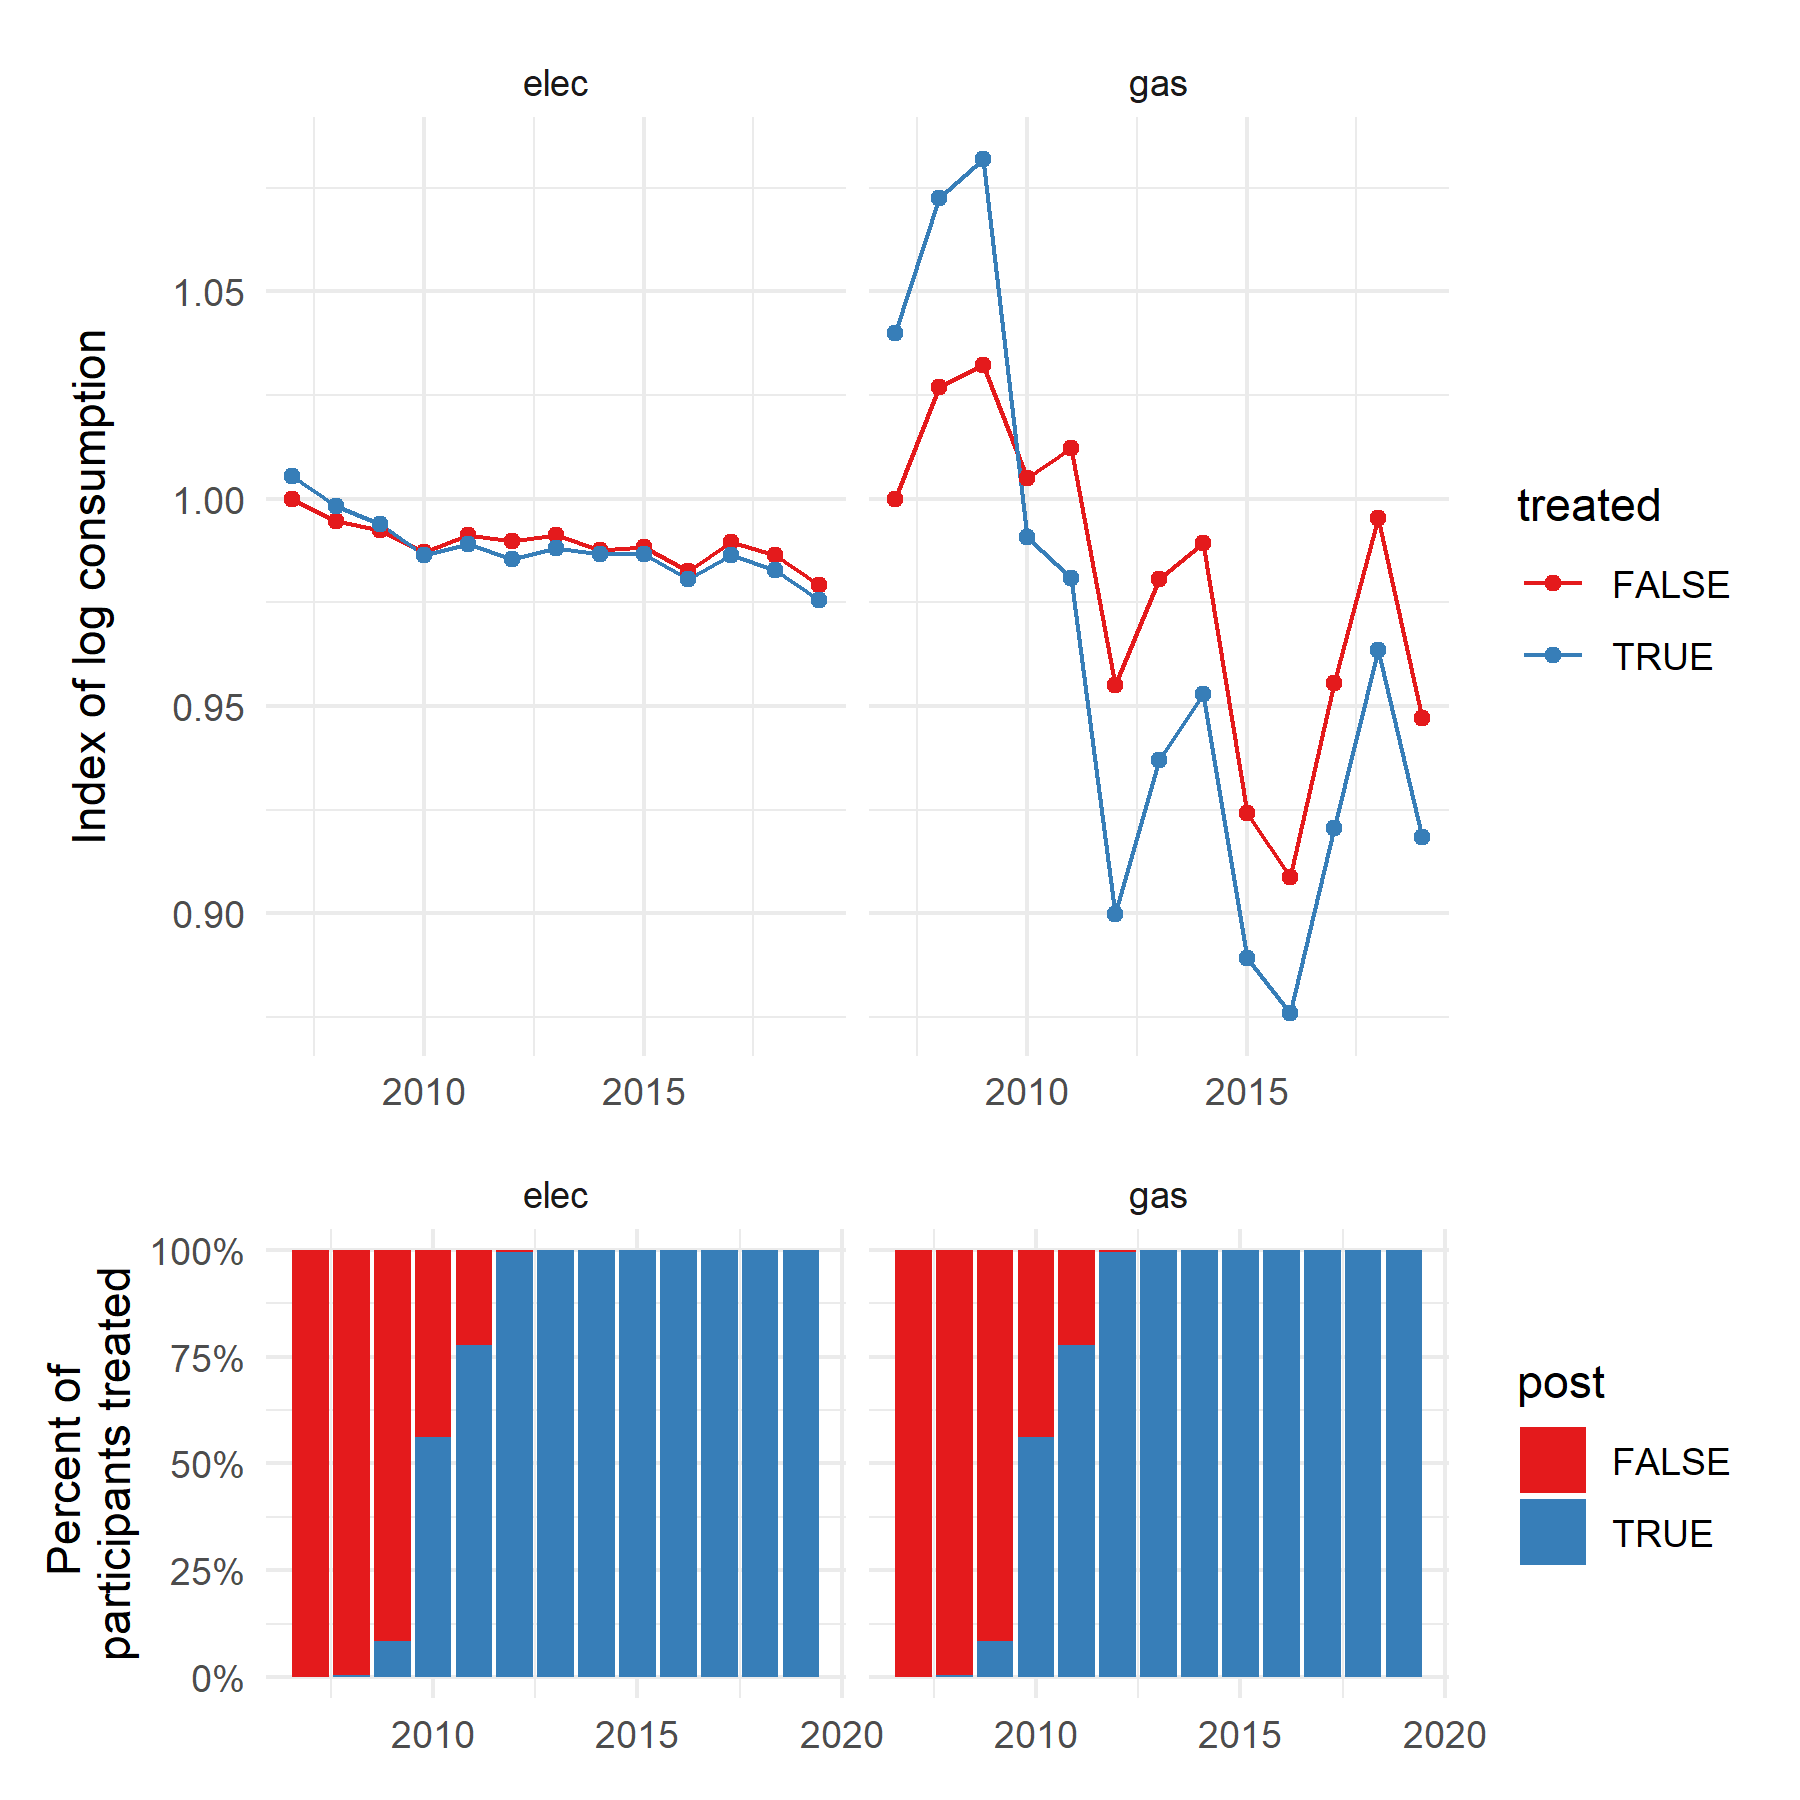
\includegraphics{../output_figures_tables/aggregate_trend_graph}
	\caption{Long-run trends in electricity and natural gas consumption in treated and untreated households}\label{fig_agg}
\end{figure}

{\color{red} Not clear to me why the aggregate trends graph suggests a gas savings of about 10\%, but we are estimating more like 20\%.}

\subsection{Regression analysis of overall energy savings}
To estimate the overall impact of participation in the energy efficiency retrofit program, we regress monthly energy consumption on an post $\times$ treatment indicator, and include household and month-of-sample fixed effects.  We consider different estimating samples:
\begin{itemize}
	\item An ever-treated sample. In this sample, we only include households that participated in the retrofit program, since these households may be more comparable to one another than non-participants. The roll-out of the program was between 2009 and 2012. We thus drop years 2012 and following. This leaves households that participated in the program in 2012 as our never-treated comparison group of participants.
	\item All households, before 2012. In this sample, we include both participating and non-participating households. We restrict the sample to exclude years 2012 and after to obtain an estimate over a similar timeframe as the never-treated sample.
	\item All households. In this sample, we include both participating and non-participating households, and include data up to 2019, which allows us to observe households for up to 11 years following initial treatment.
\end{itemize}
In all cases, we cluster standard errors on both household as well as month-of-sample.  The table below shows estimates of total energy (gas plus electricity) savings under each of the different samples.  Column 1 is the ever-treated sample, column 2 is all households before 2012, and column 3 is all households up to 2019.  Using the ever-treated sample, we find that participation in retrofits results in roughly a 10\% reduction in household energy use. When we include the non-treated households, our estimate increases in size, to around 14\%.  The long-run and short-run results with the full set of households are roughly the same, suggesting that energy savings from retrofits persist for 10 years following implementation.


\begin{tabular}{lccc}
   \tabularnewline\midrule\midrule
   Dependent Variable: & \multicolumn{3}{c}{log(energy)}\\
   Model:             & (1)             & (2)             & (3)\\
   \midrule \emph{Variables} &   &   &  \\
   treated\_postTRUE & -0.1038$^{***}$ & -0.1451$^{***}$ & -0.1376$^{***}$\\
                      & (0.0089)        & (0.0074)        & (0.0065)\\
   \midrule \emph{Fixed-effects} &   &   &  \\
   id                 & Yes             & Yes             & Yes\\
   cons\_date        & Yes             & Yes             & Yes\\
   \midrule \emph{Fit statistics} &   &   &  \\
   Observations       & 89,118          & 1,178,183       & 3,172,442\\
   R$^2$              & 0.81032         & 0.80096         & 0.78444\\
   Within R$^2$       & 0.00717         & 0.00217         & 0.00208\\
   \midrule\midrule\multicolumn{4}{l}{\emph{Clustered (id \& cons\_date) standard-errors in parentheses}}\\
   \multicolumn{4}{l}{\emph{Signif. Codes: ***: 0.01, **: 0.05, *: 0.1}}\\
\end{tabular}



\begin{tabular}{lccc}
   \tabularnewline\midrule\midrule
   Dependent Variable: & \multicolumn{3}{c}{log(energy)}\\
   Model:             & (1)             & (2)             & (3)\\
   \midrule \emph{Variables} &   &   &  \\
   treated\_postTRUE & -0.1038$^{***}$ & -0.1451$^{***}$ & -0.1376$^{***}$\\
                      & (0.0089)        & (0.0074)        & (0.0065)\\
   \midrule \emph{Fixed-effects} &   &   &  \\
   id                 & Yes             & Yes             & Yes\\
   cons\_date        & Yes             & Yes             & Yes\\
   \midrule \emph{Fit statistics} &   &   &  \\
   Observations       & 89,118          & 1,178,183       & 3,172,442\\
   R$^2$              & 0.81032         & 0.80096         & 0.78444\\
   Within R$^2$       & 0.00717         & 0.00217         & 0.00208\\
   \midrule\midrule\multicolumn{4}{l}{\emph{Clustered (id \& cons\_date) standard-errors in parentheses}}\\
   \multicolumn{4}{l}{\emph{Signif. Codes: ***: 0.01, **: 0.05, *: 0.1}}\\
\end{tabular}




\subsection{Staggered adoption and event studies}
One potential reason for the difference in results with the ever-treated and never-treated samples is because adoption of the energy efficiency measures is staggered over time. Because of the small control group in the ever-treated sample (only a few households retrofit in 2012, and these form the control group in that sample), a large weight is placed on comparisons between newly-treated and previously-treated households. Many papers suggest that these comparisons are potentially problematic, and can result in bias.  We thus conduct our estimation with alternative estimators from Callaway and Sant'a Anna and from Sun and Abraham.  We show results in the form of an event study plot, Figure \ref{fig_esplot}.

The results suggest that the TWFE estimates including the never treated households match well with the Callaway and Sant'a Anna and Sun and Abraham results.  In contrast, the ever-treated sub-sample appears to result in significantly biased coefficients.

\begin{figure}
	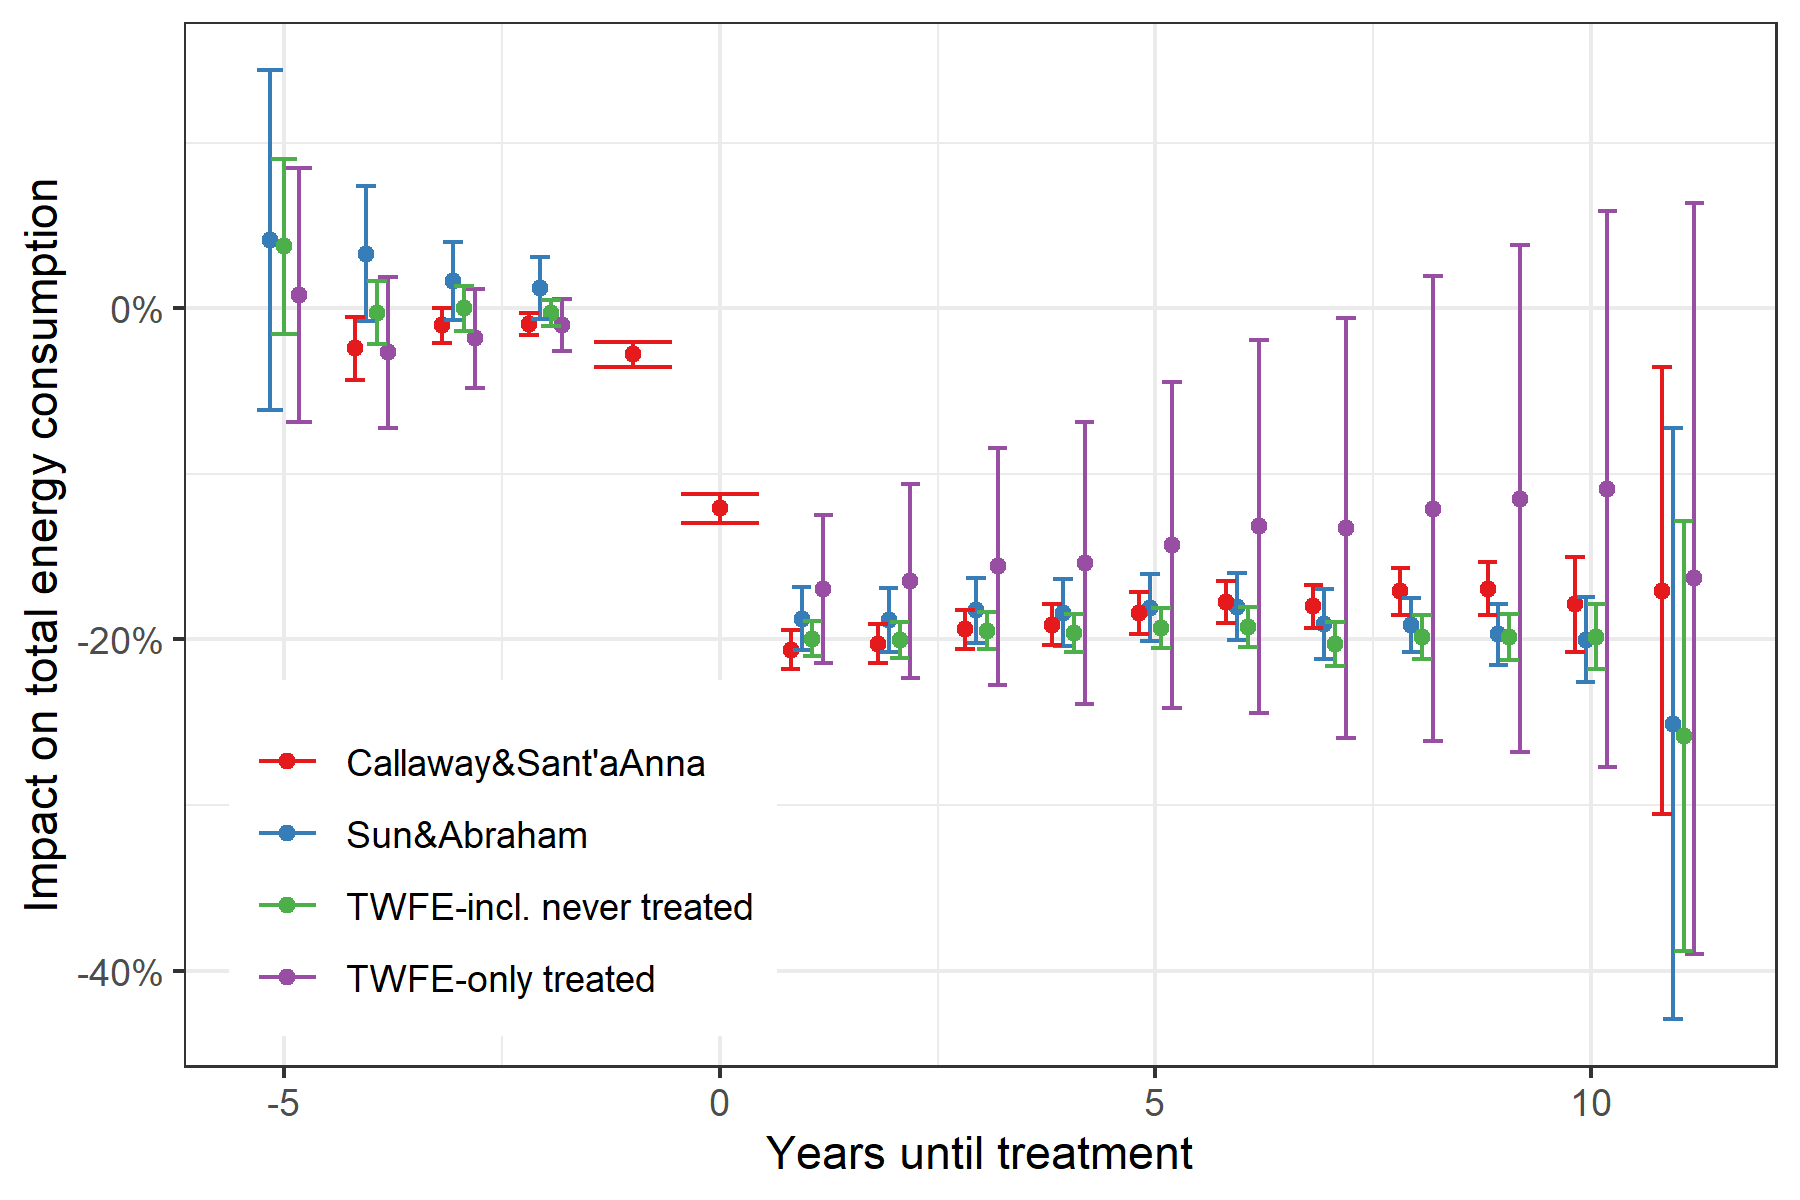
\includegraphics{../output_figures_tables/event_study_plot}
	\caption{Event study plot with different estimation samples and methods}\label{fig_esplot}
\end{figure}


\subsection{Measure specific results}

\subsubsection{Which energy efficiency measures are adopted?}
To estimate projected savings associated with different energy efficiency retrofits, we regress projected energy savings on a vector of dummy variables that indicate whether a measure was implemented:
\begin{align}
	\log y^1_i - \log y^0_i = \sum_j \beta_j x_{ij}.
\end{align}
In the equation, $y^1_i$ is the projected energy consumption of house $i$ after a retrofit is undertaken and $y^0_i$ is projected energy consumption before the retrofit is undertaken. $x_{ij}$ is a dummy variable indicating whether house $i$ implemented retrofit $j$.

Before presenting the results, Figure \ref{fig_corplot} shows a correlation plot of energy efficiency measures. If adoption of measures is highly correlated, it may be difficult to precisely estimate energy savings.  Figure \ref{fig_corplot} shows that for the most part, there is limited correlation between measures.  Only basement insulation and foundation headers are highly correlated.  It may make sense to aggregate these two measures (I haven't done this).

\begin{figure}
	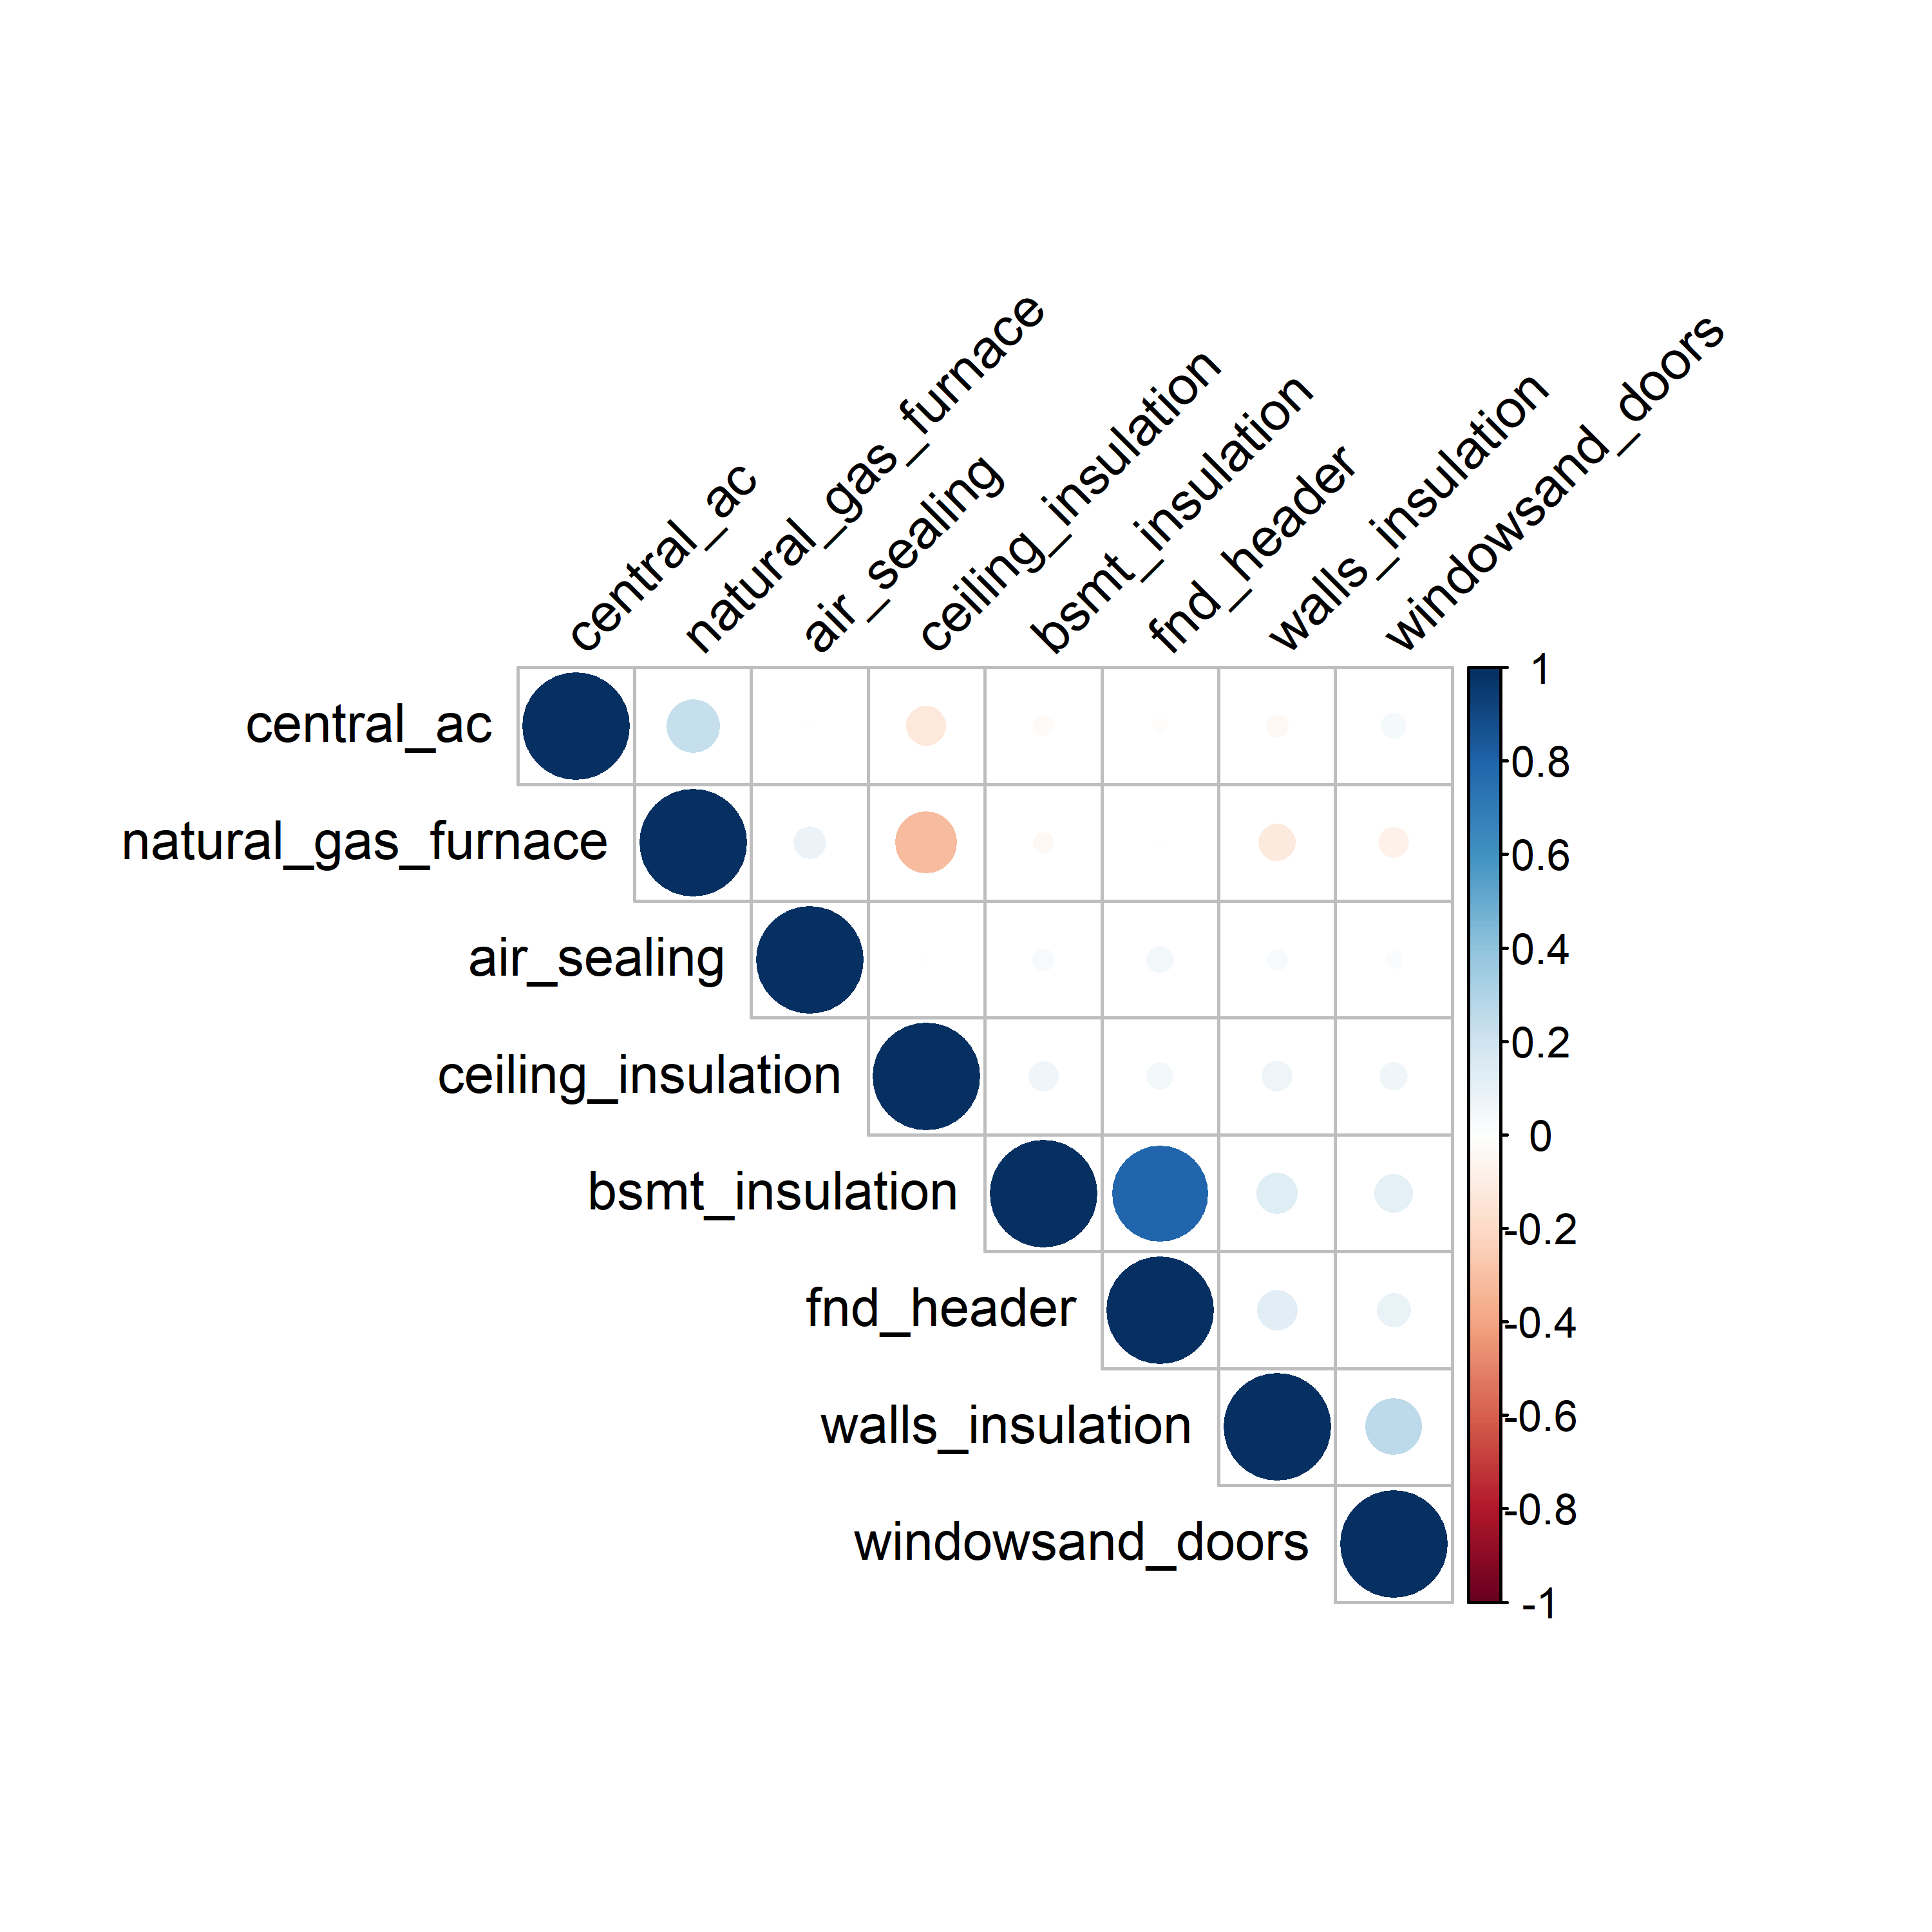
\includegraphics{"../output_figures_tables/correlation_plot.png"}
	\caption{Correlation plot of retrofit measures}\label{fig_corplot}
\end{figure}

Figure \ref{fig_mbm_proj} shows projections of energy savings by measure. Large savings are projected for natural gas furnace upgrades as well as wall insulation.

\begin{figure}
	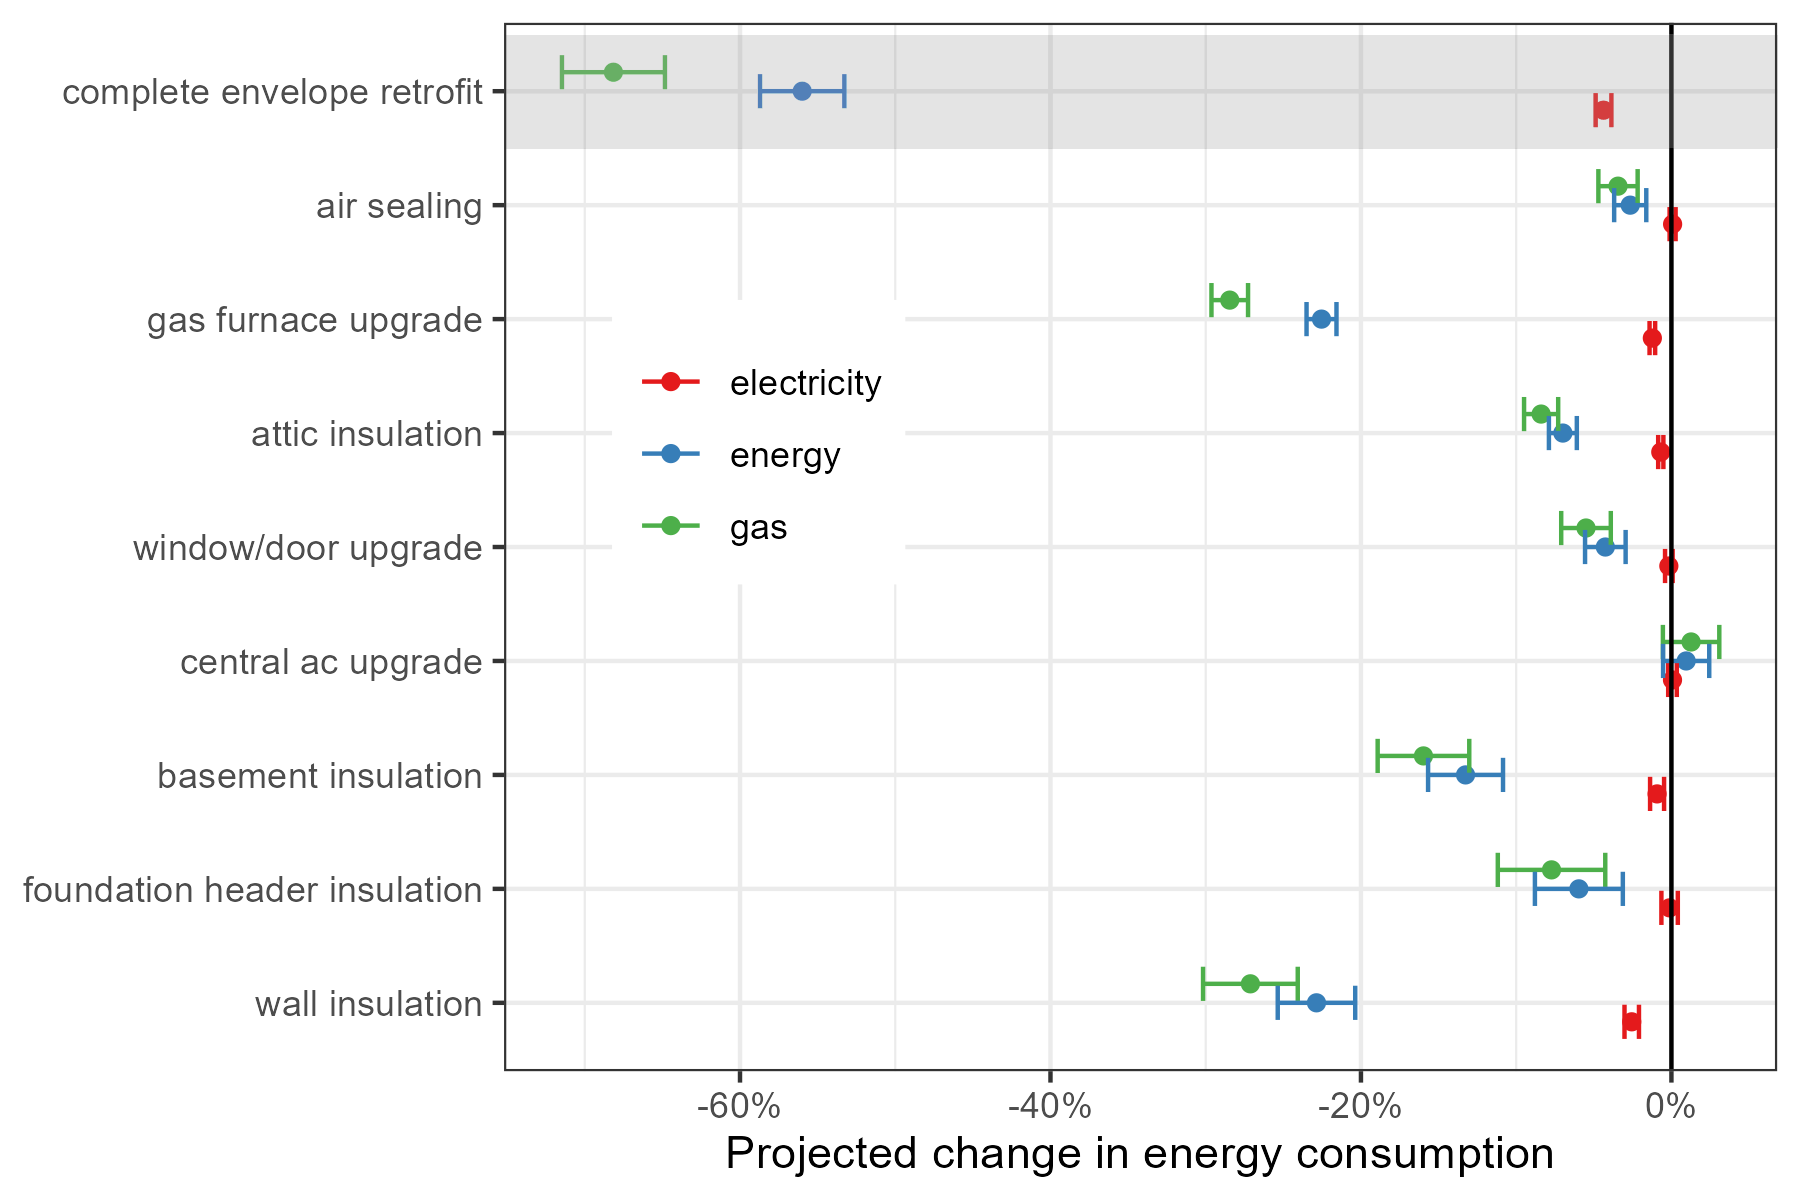
\includegraphics{../output_figures_tables/projected_es_mbm.png}
	\caption{Measure-specific energy saving projections}\label{fig_mbm_proj}
\end{figure}


\subsubsection{Estimated savings}

Figure \ref{fig_proj} shows estimated energy savings from different adopted measures (left panel) and the number of measures adopted (right panel). The largest estimated changes in gas consumption are largest for natural gas furnace upgrades and wall insulation. Air sealing and attic (ceiling) insulation also deliver gas savings that are precisely estimated. In contrast, no measure is shown to save electricity, and walls insulation may actually increase electricity consumption (although few houses adopt walls insulation).

\begin{figure}
	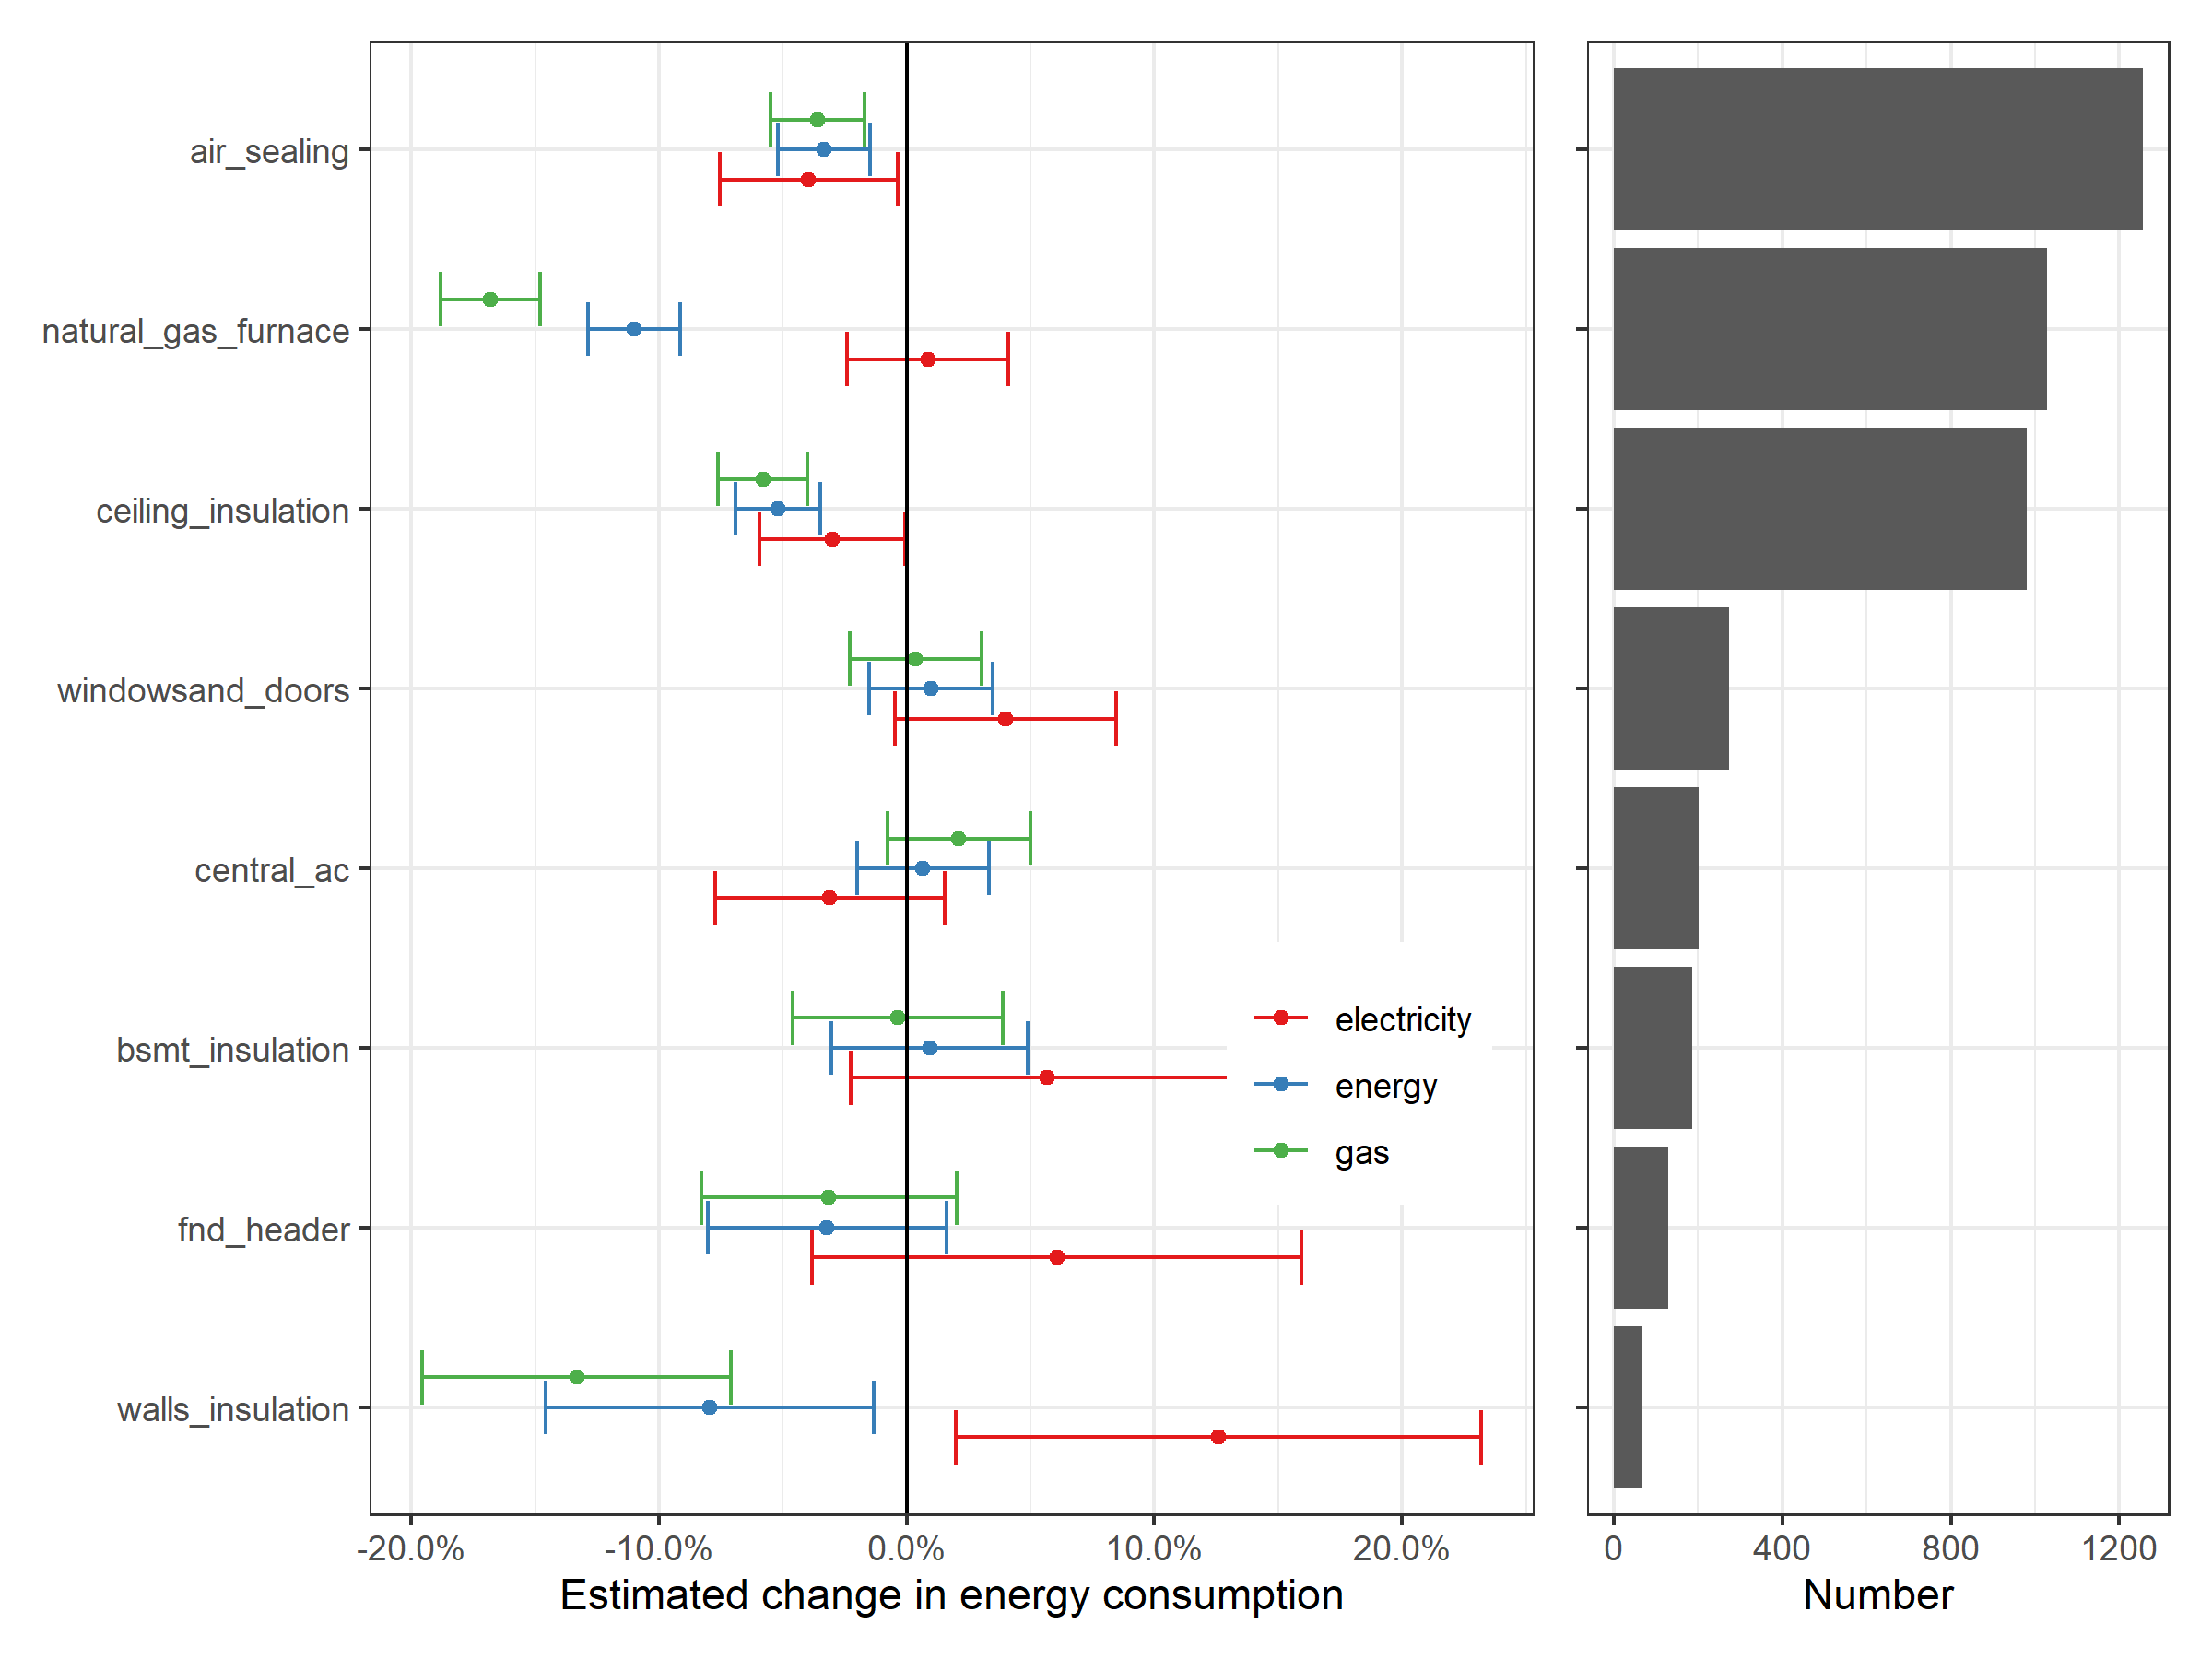
\includegraphics[width=\linewidth]{../output_figures_tables/mbm_energy_savings_combined.png}
	\caption{Estimated energy savings}\label{fig_proj}
\end{figure}


\subsubsection{Realization rates}
We estimate an aggregate realization rate by regressing energy consumption on a post $\times$ treatment dummy interacted with projected energy savings. As shown in the table below, we find a realization rate for natural gas of 50\%. Our realization rate for electricity is negative (we find an increase in electricity consumption, rather than a saving). For all energy, we find a realization rate of 47\%.


\begin{tabular}{lccc}
   \tabularnewline\midrule\midrule
   Dependent Variables:                                & log(gas)       & log(elec)             & log(energy)\\
   Model:                                              & (1)            & (2)                   & (3)\\
   \midrule \emph{Variables} &   &   &  \\
   as.numeric(treated\_post) $\times$ delta\_gas    & 0.6055$^{***}$ &                       &   \\
                                                       & (0.0195)       &                       &   \\
   as.numeric(treated\_post) $\times$ delta\_elec   &                & 0.1226                &   \\
                                                       &                & (0.5118)              &   \\
   as.numeric(treated\_post) $\times$ delta\_energy &                &                       & 0.5464$^{***}$\\
                                                       &                &                       & (0.0276)\\
   \midrule \emph{Fixed-effects} &   &   &  \\
   id                                                  & Yes            & Yes                   & Yes\\
   cons\_date                                         & Yes            & Yes                   & Yes\\
   \midrule \emph{Fit statistics} &   &   &  \\
   Observations                                        & 3,165,406      & 3,208,330             & 3,176,199\\
   R$^2$                                               & 0.84913        & 0.47322               & 0.78446\\
   Within R$^2$                                        & 0.00417        & $4.62\times 10^{-7}$ & 0.00258\\
   \midrule\midrule\multicolumn{4}{l}{\emph{Clustered (id \& cons\_date) standard-errors in parentheses}}\\
   \multicolumn{4}{l}{\emph{Signif. Codes: ***: 0.01, **: 0.05, *: 0.1}}\\
\end{tabular}




We also conduct our analysis in levels rather than logs. Results are shown in the table below, an are similar to the main results in logs.


\begin{tabular}{lccc}
   \tabularnewline\midrule\midrule
   Dependent Variables:                                      & gas            & elec                  & energy\\
   Model:                                                    & (1)            & (2)                   & (3)\\
   \midrule \emph{Variables} &   &   &  \\
   as.numeric(treated\_post) $\times$ delta\_gas\_lev    & 0.6245$^{***}$ &                       &   \\
                                                             & (0.0661)       &                       &   \\
   as.numeric(treated\_post) $\times$ delta\_elec\_lev   &                & 0.0499                &   \\
                                                             &                & (0.4932)              &   \\
   as.numeric(treated\_post) $\times$ delta\_energy\_lev &                &                       & 0.4970$^{***}$\\
                                                             &                &                       & (0.0553)\\
   \midrule \emph{Fixed-effects} &   &   &  \\
   id                                                        & Yes            & Yes                   & Yes\\
   cons\_date                                               & Yes            & Yes                   & Yes\\
   \midrule \emph{Fit statistics} &   &   &  \\
   Observations                                              & 3,192,857      & 3,210,277             & 3,176,946\\
   R$^2$                                                     & 0.75198        & 0.54135               & 0.74822\\
   Within R$^2$                                              & 0.00360        & $1.43\times 10^{-7}$ & 0.00327\\
   \midrule\midrule\multicolumn{4}{l}{\emph{Clustered (id \& cons\_date) standard-errors in parentheses}}\\
   \multicolumn{4}{l}{\emph{Signif. Codes: ***: 0.01, **: 0.05, *: 0.1}}\\
\end{tabular}




Finally, we estimate measure specific realization rates by dividing realized by projected energy savings by measure.  Results are presented in Figure \ref{fig_rr_mbm}. We indicate measure-specific realization rates in percentage form above each measure. For natural gas, we find realizatoin rates of 59\% for furnace upgrades and 51\% for walls insulation. We find a realization rate of above 100\% for air sealing measures. For electricity, we find realization rates that are mostly negative, since most measures appear to be associated with an increase in electricity consumption.

\begin{figure}
	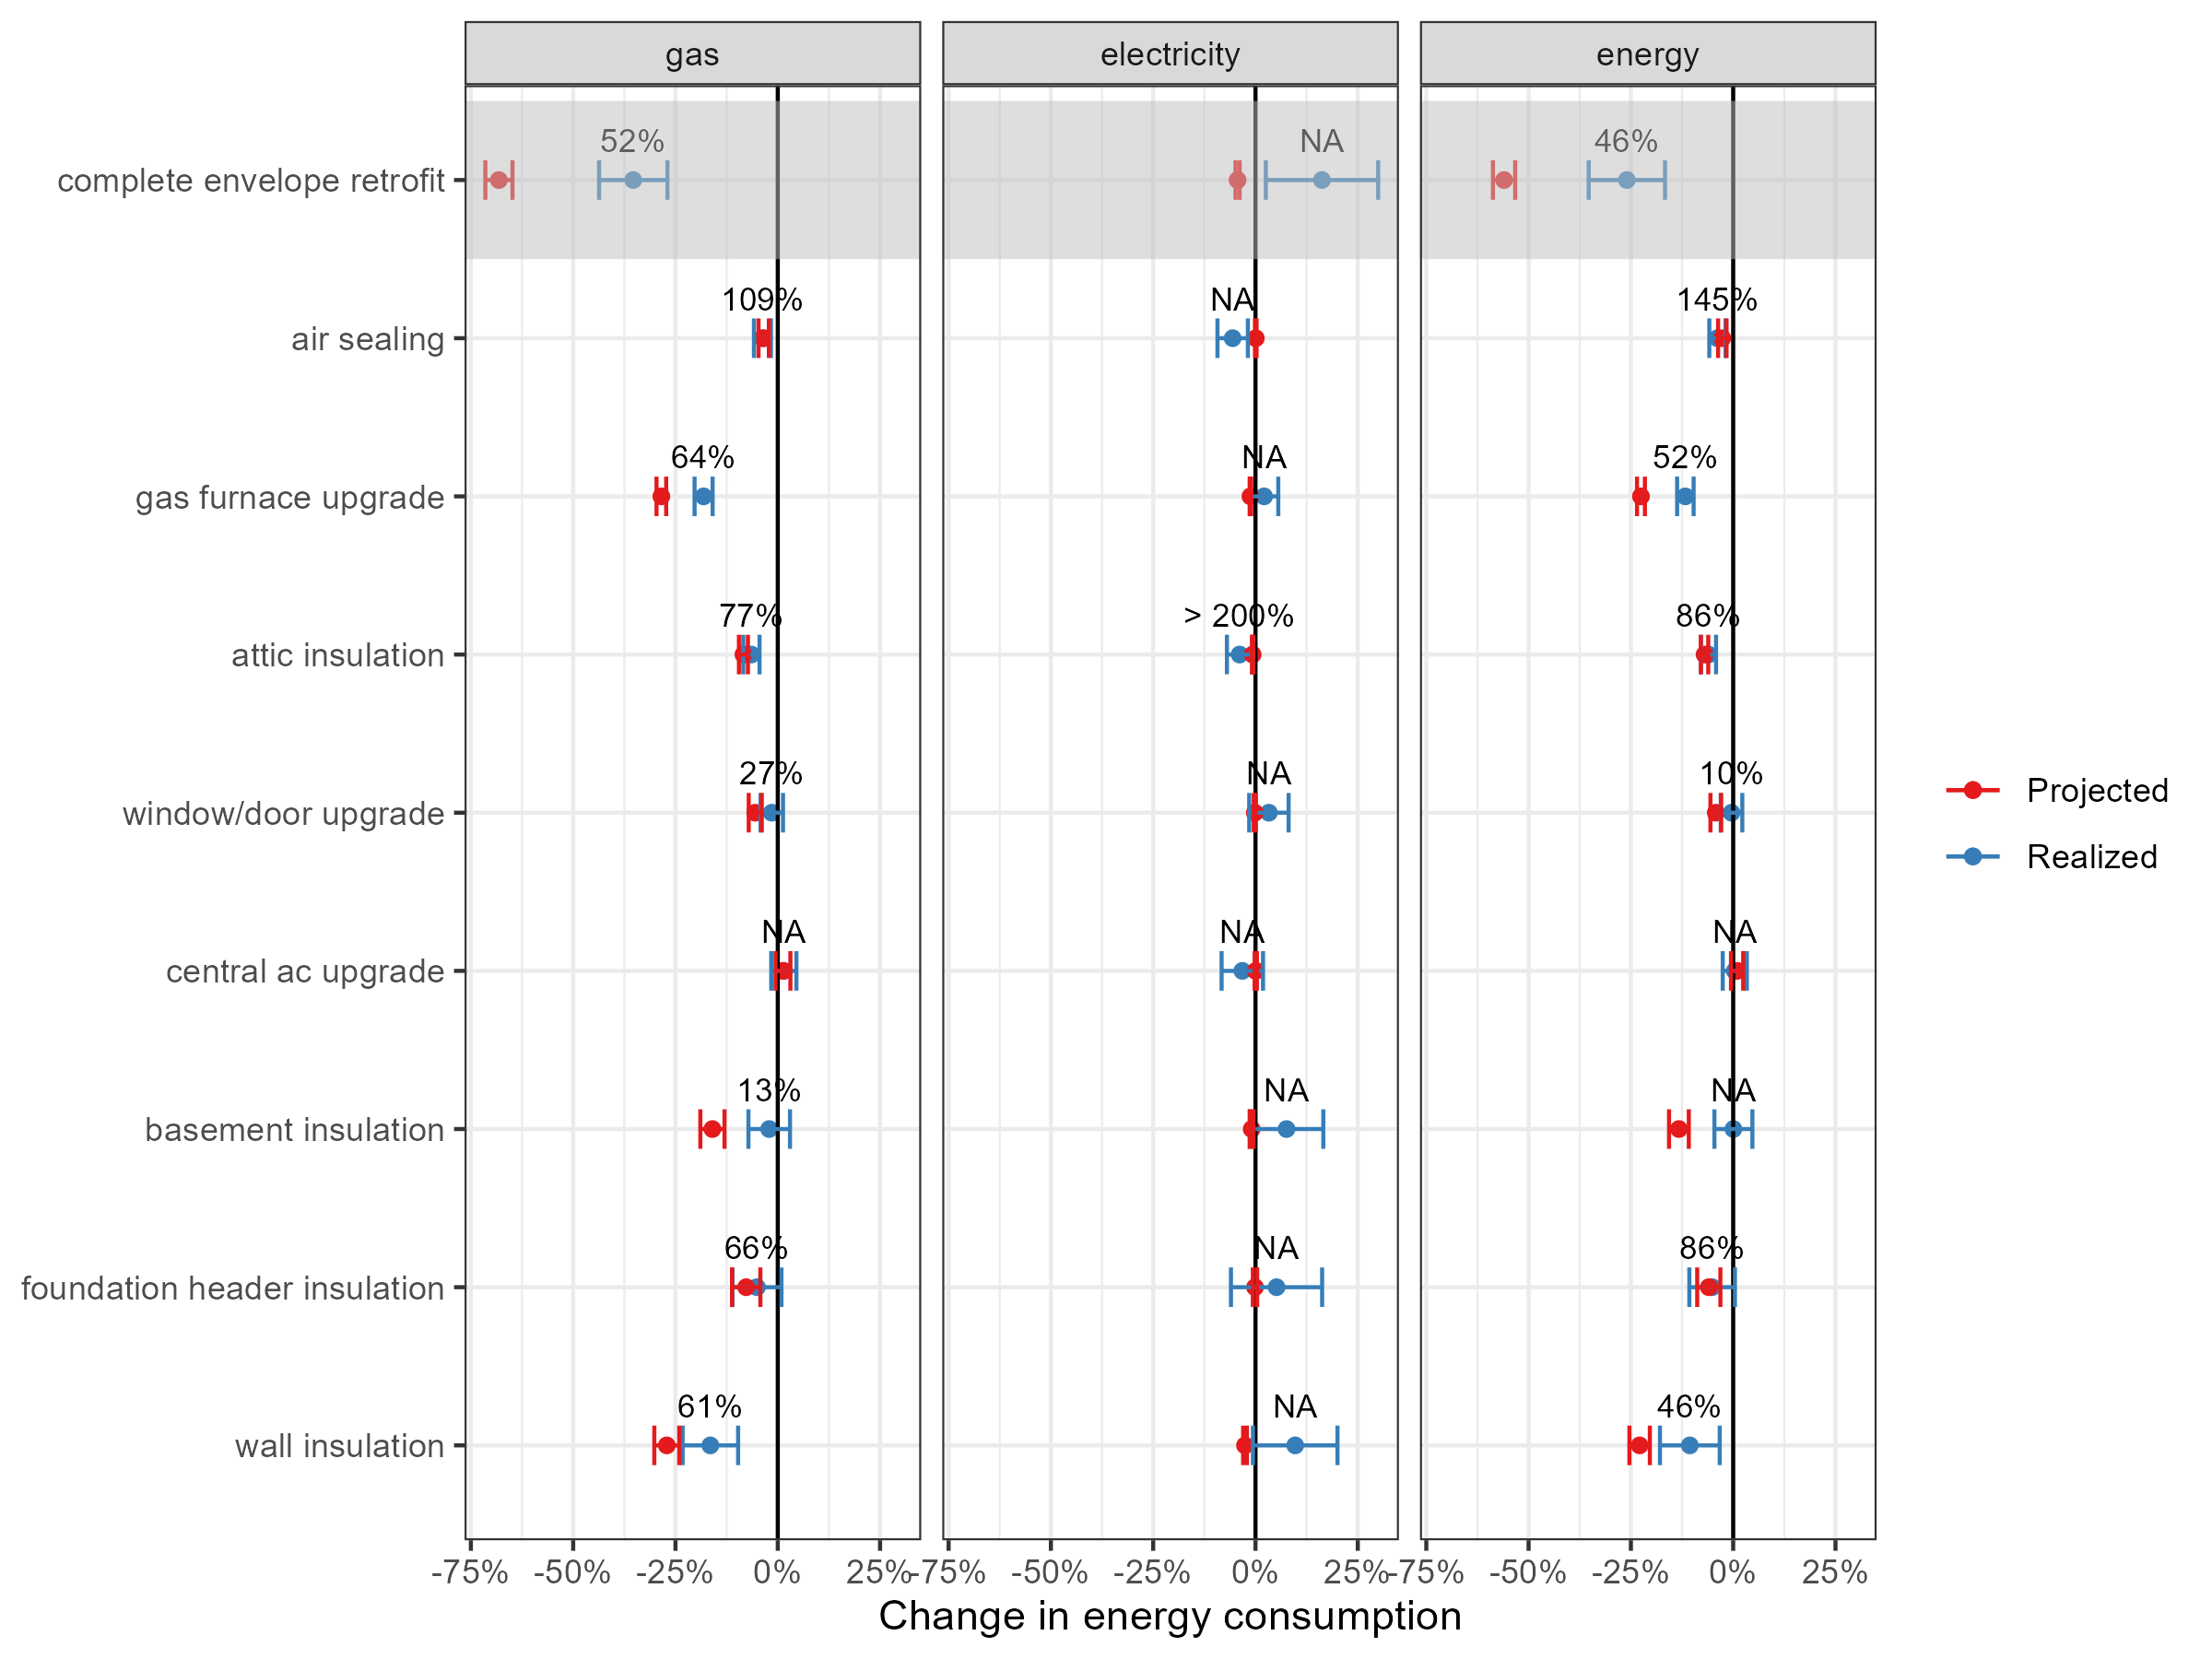
\includegraphics[width=\linewidth]{../output_figures_tables/mbm_realization_rate.png}
	\caption{Measure specific realization rates}\label{fig_rr_mbm}
\end{figure}

\section{Conclusion}


\end{document}